\documentclass[12pt,a4paper]{article}

% =========================
% PACKAGES
% =========================
\usepackage[utf8]{inputenc}
\usepackage[T5]{fontenc}
\usepackage[provide=*,vietnamese]{babel}
\usepackage{geometry}
\usepackage{array}
\usepackage{longtable}
\usepackage{booktabs}
\usepackage{multirow}
\usepackage{graphicx}
\usepackage{xcolor}
\usepackage{hyperref}
\usepackage{enumitem}
\usepackage{listings}
\usepackage{fancyhdr}
\usepackage{titlesec}
\usepackage{tabularx}
\usepackage{pgfplots}
\usepackage{tikz}
\usetikzlibrary{shapes.geometric, arrows.meta, positioning, calc}
\pgfplotsset{compat=1.18}

% =========================
% SETTINGS & STYLES
% =========================
\geometry{
    left=2.5cm,
    right=2.5cm,
    top=2.5cm,
    bottom=2.5cm
}

\hypersetup{
    colorlinks=true,
    linkcolor=darkblue,
    urlcolor=darkblue,
    citecolor=darkblue
}

\definecolor{lightgray}{gray}{0.96}
\definecolor{darkblue}{RGB}{0, 70, 140}
\definecolor{darkred}{RGB}{150, 20, 20}
\definecolor{darkgreen}{RGB}{20, 120, 60}

\lstdefinestyle{codestyle}{
    backgroundcolor=\color{lightgray},
    basicstyle=\ttfamily\small,
    breaklines=true,
    frame=single,
    columns=fullflexible
}

% Định dạng cho TikZ Diagram
\tikzset{
    box/.style = {rectangle, draw=darkblue, fill=white, thick, text width=3.5cm, align=center, rounded corners, minimum height=1cm},
    widebox/.style = {rectangle, draw=darkblue, fill=white, thick, text width=6.5cm, align=center, rounded corners, minimum height=1cm},
    decision/.style = {diamond, draw=darkred, fill=white, thick, text width=2.5cm, align=center, inner sep=-2pt},
    arrow/.style = {thick, ->, >=stealth},
    line/.style = {thick, -}
}

\pagestyle{fancy}
\fancyhf{}
\lhead{\footnotesize Clinical Ambient Documentation Assistant}
\rhead{\footnotesize Báo cáo Kỹ thuật Đợt 2}
\cfoot{\thepage}

\titleformat{\section}
{\normalfont\Large\bfseries\color{darkblue}}
{\thesection}{1em}{}

\titleformat{\subsection}
{\normalfont\large\bfseries\color{darkblue}}
{\thesubsection}{1em}{}

\title{
    \textbf{Báo cáo Kỹ thuật Đợt 2}\\
    \large Tiền xử lý Âm thanh (Audio Preprocessing), Thực nghiệm ASR và Phân tích Rủi ro Lâm sàng\\
    \normalsize Dự án: Local-first Clinical Ambient Documentation Assistant for Vietnamese Outpatient Care
}

\author{Duy Vũ}
\date{\today}

\begin{document}

\maketitle

\begin{abstract}
Báo cáo đợt 2 trình bày kiến trúc và kết quả thực nghiệm của phân hệ tiền xử lý âm thanh (Audio Preprocessing) và hệ thống Nhận dạng Giọng nói Tự động (ASR) áp dụng cho hồ sơ y tế ngoại trú tiếng Việt. Tiếp nối chiến lược quản trị dữ liệu từ đợt 1, đợt này tập trung vào việc thiết lập các đường ống (pipeline) kỹ thuật: từ khâu nhập liệu (ingestion) bộ dữ liệu VietMed, chuẩn hóa định dạng tín hiệu âm thanh thông qua kịch bản \texttt{normalize\_public\_audio.py}, phân chia tập dữ liệu nghiêm ngặt dựa trên bản quyền bằng \texttt{create\_asr\_splits.py}, cho đến đánh giá thực nghiệm (benchmark) trên nền tảng Google Colab.

Kết quả đánh giá trên tập phát triển (Dev split - 200 mẫu) cho thấy mô hình pre-trained \texttt{vinai/PhoWhisper-medium} đạt hiệu suất khả quan nhất với Tỷ lệ Lỗi Từ được chuẩn hóa (Normalized WER) là 21.51\%, tiệm cận mục tiêu kỹ thuật ($< 20\%$). Tuy nhiên, phân tích sâu về phương diện an toàn lâm sàng bộc lộ các hạn chế liên quan đến lỗi mất từ phủ định (Negation deletion) và sai lệch thuật ngữ y khoa. Báo cáo đề xuất phương án tinh chỉnh (fine-tuning) có kiểm soát trong giai đoạn tiếp theo nhằm cải thiện không chỉ độ chính xác từ vựng mà còn tối ưu hóa tính an toàn y tế trong hệ thống tài liệu hóa lâm sàng.
\end{abstract}

\tableofcontents
\newpage

% ======================================================
\section{Tóm tắt Điều hành}

\subsection{Mục tiêu báo cáo}

Mục tiêu cốt lõi của giai đoạn này là chuyển dịch từ nghiên cứu lý thuyết sang triển khai và đo lường thực nghiệm đối với bài toán ASR y khoa tiếng Việt. Quá trình này đòi hỏi một quy trình đánh giá minh bạch, có khả năng tái lập và tuân thủ các nguyên tắc quản trị dữ liệu y tế:
\begin{itemize}[leftmargin=1.2cm]
    \item \textbf{Data Ingestion:} Tích hợp bộ dữ liệu VietMed vào các phân vùng lưu trữ Bronze và Silver.
    \item \textbf{Audio Normalization:} Chuẩn hóa tần số lấy mẫu (sample rate) và số kênh (channels) nhằm tối ưu độ trích xuất đặc trưng của ASR.
    \item \textbf{Data Splitting:} Cô lập tập huấn luyện, phát triển và kiểm thử (Train/Dev/Test) có kiểm soát chặt chẽ.
    \item \textbf{Benchmarking:} Đánh giá trên nền tảng Google Colab các mô hình ngôn ngữ lớn xử lý giọng nói (Whisper, PhoWhisper).
    \item \textbf{Clinical Error Analysis:} Phân tích định tính các lỗi nghiêm trọng về lâm sàng (phủ định, liều lượng, thuật ngữ y khoa) bên cạnh các chỉ số định lượng như Strict/Normalized WER.
\end{itemize}

\subsection{Kết quả Nổi bật}

\begin{table}[h]
\centering
\caption{Tổng quan kết quả thực nghiệm ASR Baseline}
\begin{tabularx}{\textwidth}{|l|X|}
\hline
\textbf{Chỉ tiêu đánh giá} & \textbf{Kết quả ghi nhận} \\
\hline
Mô hình đạt hiệu năng cao nhất & \texttt{vinai/PhoWhisper-medium} \\
\hline
Normalized WER tối ưu & 21.51\% \\
\hline
Strict WER tương ứng & 24.64\% \\
\hline
Quy mô dữ liệu đánh giá & 200 mẫu ghi âm thuộc tập Dev (VietMed) \\
\hline
Tốc độ suy luận (Inference time) & $\approx$ 0.42 giây/mẫu (Google Colab - GPU T4) \\
\hline
Trạng thái mô hình & Pre-trained (Chưa tiến hành Fine-tuning) \\
\hline
Mục tiêu giai đoạn kế tiếp & Giảm Normalized WER $< 20\%$ và triệt tiêu lỗi phủ định (Negation Errors). \\
\hline
\end{tabularx}
\end{table}

Chỉ số Normalized WER đạt 21.51\% minh chứng cho khả năng học chuyển giao (transfer learning) tốt của mô hình cơ sở. Mặc dù kết quả tiệm cận ngưỡng mục tiêu, đặc thù y khoa đòi hỏi khắt khe hơn về độ an toàn thông tin. Một transcript có tỷ lệ lỗi tổng thể thấp vẫn hoàn toàn có khả năng gây rủi ro y khoa nếu nhận diện sai hoặc lược bỏ các từ khóa phủ định hay tên thuốc.

% ======================================================
\section{Bối cảnh \& Nền tảng Kỹ thuật}

\subsection{Kế thừa từ giai đoạn trước}

Giai đoạn 1 đã xác lập ba trụ cột nền tảng cho dự án:
\begin{enumerate}[leftmargin=1.2cm]
    \item \textbf{Data Governance:} Nguyên tắc quản trị dữ liệu đảm bảo tính tuân thủ trong AI y tế.
    \item \textbf{Synthetic Data Pipeline:} Giao thức "Gold Standard" tạo dữ liệu lâm sàng tổng hợp (\texttt{SYN\_OUT\_00X}).
    \item \textbf{Algorithm Research:} Đánh giá kiến trúc Transformer ứng dụng trong Whisper/PhoWhisper.
\end{enumerate}

Giai đoạn 2 kế thừa các nguyên tắc này, hiện thực hóa chúng qua mã nguồn Python chuẩn mực và chạy thực nghiệm định lượng, đồng thời giải quyết các bài toán về tối ưu hóa chi phí điện toán bằng cách triển khai quy trình đánh giá trên Google Colab.

\subsection{Tầm quan trọng của Audio Preprocessing}

Trong kiến trúc đường ống (pipeline) Nhận dạng Giọng nói, tiền xử lý âm thanh (Audio Preprocessing) không chỉ là một bước phụ trợ mà là phân hệ thiết yếu, đóng vai trò bản lề quyết định toàn bộ chất lượng của hệ thống downstream. Đặc thù của môi trường phòng khám ngoại trú (outpatient care) thường lẫn nhiều tạp âm (tiếng quạt, tiếng bước chân, giọng nói nền), khiến tín hiệu thu được rất đa dạng về dải động và chất lượng.
\begin{itemize}[leftmargin=1.2cm]
    \item \textbf{Mô hình ASR:} Các kiến trúc dựa trên Transformer như Whisper được huấn luyện chủ yếu trên phổ âm thanh 16kHz. Chúng cực kỳ nhạy cảm với sự biến thiên tần số lấy mẫu (sample rate) và dải động (dynamic range). Một tín hiệu đầu vào không chuẩn hóa có thể khiến tầng tích chập (convolutional layers) trích xuất sai đặc trưng Mel-spectrogram.
    \item \textbf{Mô đun Phân mảnh (Diarization):} Trong tương lai, việc tách giọng bác sĩ và bệnh nhân sẽ dễ bị ảnh hưởng bởi nhiễu nền hoặc khoảng lặng bất thường nếu mức năng lượng tín hiệu (volume) không được cân bằng.
    \item \textbf{Trích xuất Sự kiện Lâm sàng (Clinical NLP):} Bị sai lệch dây chuyền (cascading failure). Nếu âm thanh đầu vào kém khiến ASR nhận diện sai một từ khóa, hệ thống NLP phía sau sẽ trích xuất sai sự kiện y khoa (Clinical Fact), dẫn đến hồ sơ bệnh án SOAP bị sai lệch hoàn toàn.
\end{itemize}
Vì vậy, Audio Preprocessing tại dự án được chuẩn hóa bằng mã nguồn tự động để đảm bảo độ tái lập 100\%, đồng thời tạo ra một baseline vững chắc cho các thử nghiệm mô hình.

% ======================================================
\section{Kiến trúc Đường ống Dữ liệu \& Tiền xử lý}

\subsection{Luồng Dữ liệu và Tiêu chí Quản trị (Data Lake Governance)}

Nhằm đảm bảo tuân thủ nghiêm ngặt các nguyên tắc bảo mật thông tin y tế (PHI) và chuẩn hóa dữ liệu đầu vào, hệ thống triển khai kiến trúc Cổng quản trị (Governance Gate) trước khi dữ liệu được đưa vào xử lý.

\begin{figure}[h]
\centering
\resizebox{0.95\textwidth}{!}{
\begin{tikzpicture}[node distance=1cm and 1cm]
% Nodes
\node (A) [widebox] {Nguồn dữ liệu (Data Sources)};
\node (sources) [widebox, below=of A, yshift=0.5cm] {
    \begin{tabular}{ll}
    $\bullet$ Synthetic/simulated audio & $\bullet$ Clinical fact annotation \\
    $\bullet$ Approved real audio & $\bullet$ Doctor review logs \\
    $\bullet$ Manual transcript & $\bullet$ Medical dictionary v0.1 \\
    $\bullet$ Speaker annotation & $\bullet$ Model outputs
    \end{tabular}
};

\node (B) [decision, below=of sources, yshift=0cm, aspect=2.5, inner sep=0pt, text width=3.5cm] {Privacy \&\\Governance Gate};

\node (checks) [widebox, right=of B, xshift=1.5cm] {
    \begin{tabular}{c}
    Consent / approval check \\
    PII / PHI handling
    \end{tabular}
};

\node (C) [box, fill=orange!10, below=of B, yshift=0cm] {Bronze Zone};
\node (D) [box, fill=gray!20, below=of C, yshift=0.5cm] {Silver Zone};
\node (E) [box, fill=yellow!10, below=of D, yshift=0.5cm] {Gold Zone};

% Arrows
\draw [arrow] (A) -- (sources);
\draw [arrow] (sources) -- (B);
\draw [line, dashed] (B) -- (checks);
\draw [arrow] (B) -- node[right, font=\footnotesize] {Passed} (C);
\draw [arrow] (C) -- (D);
\draw [arrow] (D) -- (E);

\end{tikzpicture}
}
\caption{Lưu đồ Quản trị Dữ liệu (Governance Gate) và Phân vùng Data Lake}
\end{figure}

\subsection{Thiết kế Tiêu chuẩn Dữ liệu (Minimum Annotation Schema)}

Bất kỳ âm thanh khám bệnh (encounter) nào khi được đưa vào hệ thống đều phải tuân thủ thiết kế dữ liệu tối thiểu (Minimum Annotation Schema). Điều này bắt buộc hệ thống phải ghi nhận nguồn gốc (source attribution) cho từng sự kiện lâm sàng, đảm bảo tính minh bạch và khả năng truy vết trong y khoa.

\textbf{Cấu trúc JSON tối thiểu cho một Clinical Encounter:}
\begin{verbatim}
{
  "encounter_id": "UUID",
  "audio_id": "UUID_audio_file",
  "metadata": {
    "setting": "outpatient",
    "specialty": "internal_medicine",
    "language_locale": "vi-VN",
    "recording_environment": "clinic_room",
    "consent_status": "synthetic_or_approved",
    "source_type": "synthetic|public|volunteer|real_patient"
  },
  "segments": [
    {
      "segment_id": "seg_001",
      "start_time": 0.0,
      "end_time": 7.2,
      "speaker_id": "Speaker_0",
      "speaker_role": "Doctor",
      "text": "Hôm nay anh thấy khó chịu ở đâu?",
      "asr_confidence": 0.91
    }
  ],
  "clinical_facts": [
    {
      "fact_id": "fact_001",
      "type": "symptom",
      "text": "ho 3 ngày",
      "assertion": "present",
      "source_segments": ["seg_004", "seg_005"],
      "coding_candidates": [
        {
          "system": "local_dictionary",
          "code": "SYM_COUGH",
          "display": "Ho"
        }
      ],
      "requires_doctor_confirmation": true,
      "doctor_confirmation_status": "accepted|edited|rejected|pending"
    }
  ],
  "note": {
    "format": "SOAP-lite",
    "draft": "...",
    "reviewed_version": "...",
    "status": "draft|reviewed|exported"
  },
  "audit": {
    "reviewer_id": "doctor_or_simulated_reviewer",
    "correction_time_seconds": 0,
    "version": "v0.1"
  }
}
\end{verbatim}

\subsection{Kiến trúc Tổng quan Tiến trình}

Dữ liệu đi qua các vùng lưu trữ (Data Zones) được kiểm soát nghiêm ngặt. Dữ liệu công khai (Public data) phải trải qua bước tiền xử lý trước khi được công nhận là dữ liệu sạch (Silver zone).

\begin{figure}[h]
\centering
\begin{tikzpicture}[node distance=1cm and 2cm]
% Nodes
\node (A) [widebox] {Dữ liệu ASR công khai: VietMed};

\node (B) [widebox, below=of A] {Bronze Zone\\ \footnotesize (Raw audio, raw transcript, metadata, license snapshot)};

\node (C) [widebox, below=of B] {Tiền xử lý Âm thanh (\texttt{normalize\_public\_audio.py})\\ \footnotesize Chuyển đổi mono, 16kHz, chuẩn hóa âm lượng};

\node (D) [widebox, below=of C] {Silver Zone\\ \footnotesize (Clean audio WAV, ASR manifest, SHA256, duration)};

\node (E) [widebox, below=of D] {Chiến lược Phân chia (\texttt{create\_asr\_splits.py})\\ \footnotesize Train (600), Dev (200), Test (200)};

\node (F) [widebox, below=of E] {Thực nghiệm Baseline (Colab GPU T4)\\ \footnotesize (Whisper-small, PhoWhisper-base/medium)};

\node (G) [widebox, below=of F] {Đánh giá \& Phân tích\\ \footnotesize (WER/CER, Phân tích Lỗi Lâm sàng)};

% Arrows
\draw [arrow] (A) -- (B);
\draw [arrow] (B) -- (C);
\draw [arrow] (C) -- (D);
\draw [arrow] (D) -- (E);
\draw [arrow] (E) -- (F);
\draw [arrow] (F) -- (G);

\end{tikzpicture}
\caption{Kiến trúc đường ống Tiền xử lý Âm thanh và Thực nghiệm ASR}
\end{figure}

\subsection{Kỹ thuật Tiền xử lý: \texttt{normalize\_public\_audio.py}}

Kịch bản \texttt{normalize\_public\_audio.py} được triển khai nhằm tự động hóa khâu làm sạch dữ liệu, tận dụng thư viện xử lý âm thanh cấp thấp (FFmpeg backend) để đảm bảo tốc độ và độ chính xác. Mục tiêu kỹ thuật bao gồm:
\begin{itemize}[leftmargin=1.2cm]
    \item \textbf{Đồng nhất định dạng:} Chuyển đổi tất cả âm thanh đầu vào (bất kể là mp3, m4a hay wav đa kênh) về định dạng \texttt{WAV}, kênh đơn (Mono), và tần số lấy mẫu 16kHz. Kiến trúc PhoWhisper được huấn luyện chủ yếu trên phổ 16kHz; việc resample đồng bộ ngay từ đầu giúp triệt tiêu các lỗi mismatch tensor khi đưa vào mô hình, đồng thời tăng tốc độ load batch trong quá trình thực nghiệm.
    \item \textbf{Chuẩn hóa âm lượng (Audio Normalization):} Phân tích tín hiệu và áp dụng chuẩn hóa âm lượng (Loudness Normalization) để khắc phục tình trạng audio ghi âm điện thoại bị quá nhỏ hoặc bị bóp nghẹt.
    \item \textbf{Tính toàn vẹn Dữ liệu:} Sử dụng thuật toán băm mã hóa SHA-256 để tính toán checksum cho từng tệp đầu ra. Bất kỳ sự thay đổi nhỏ nào trong file âm thanh sẽ làm thay đổi chuỗi checksum, giúp hệ thống phát hiện rò rỉ dữ liệu hoặc sai lệch manifest một cách dễ dàng.
    \item \textbf{Xuất Metadata:} Tự động trích xuất metadata như thời lượng (duration), cập nhật trực tiếp vào file \texttt{asr\_silver\_manifest.jsonl} để chuẩn bị cho bước chia tách tiếp theo.
\end{itemize}

% ======================================================
\section{Chiến lược Phân chia Dữ liệu (Data Splitting)}

\subsection{Phân bổ tập dữ liệu VietMed}

Dự án áp dụng kịch bản \texttt{create\_asr\_splits.py} để lọc và phân vùng dữ liệu dựa trên tiêu chí bản quyền (đảm bảo tính CC0-1.0) và độ an toàn.

\begin{table}[h]
\centering
\caption{Phân bổ tập dữ liệu thực nghiệm VietMed}
\begin{tabular}{|l|r|p{9cm}|}
\hline
\textbf{Phân vùng (Split)} & \textbf{Số lượng} & \textbf{Vai trò kỹ thuật} \\
\hline
Silver Manifest & 1050 mẫu & Tập hợp toàn bộ dữ liệu đã qua chuẩn hóa âm thanh. \\
\hline
Train Candidate & 600 mẫu & Nguồn dữ liệu dành cho pha Fine-tuning sắp tới. Không dùng trong báo cáo đánh giá nội bộ chéo. \\
\hline
Dev Split & 200 mẫu & Tập phát triển dùng để benchmark, so sánh hiệu năng các kiến trúc và chọn model tối ưu. \\
\hline
Test Holdout & 200 mẫu & Tập kiểm thử độc lập. Tuyệt đối không dùng để tune tham số nhằm tránh rò rỉ dữ liệu (Data Leakage). \\
\hline
\end{tabular}
\end{table}

% ======================================================
\section{Nghi thức Đánh giá \& Chuẩn hóa Transcript}

\subsection{Sự cần thiết của Normalized Metrics}

Trong văn bản y khoa tiếng Việt, hiện tượng đa hình (polymorphism) trong cách ghi chép rất phổ biến.
Ví dụ:
\begin{itemize}
    \item "năm trăm miligam" so với "500 mg"
    \item "ba mươi bảy độ tám" so với "37.8 độ"
\end{itemize}
Nếu chỉ áp dụng Strict WER (Word Error Rate nguyên bản), hệ thống sẽ tính toán sai lệch khả năng thấu hiểu ngữ nghĩa của mô hình. Do đó, quy trình báo cáo sử dụng hệ thống metric kép:
\begin{enumerate}
    \item \textbf{Strict WER / CER:} Đánh giá độ chính xác tuyệt đối so với chuỗi gốc.
    \item \textbf{Normalized WER / CER:} Đánh giá sau quy trình chuẩn hóa (loại bỏ dấu câu, chuyển hóa số liệu, đơn vị y khoa) nhằm phản ánh sát nhất năng lực nắm bắt ngữ cảnh.
\end{enumerate}

% ======================================================
\section{Kết quả Thực nghiệm (Baseline Benchmark)}

\subsection{Kết quả Suy luận trên Google Colab}

Các thử nghiệm được thực thi trên môi trường Google Colab sử dụng GPU NVIDIA T4 nhằm giả lập môi trường tính toán giới hạn tài nguyên.

\begin{table}[h]
\centering
\caption{Kết quả Baseline trên tập VietMed Dev (200 mẫu)}
\resizebox{\textwidth}{!}{
\begin{tabular}{|l|c|c|c|c|l|}
\hline
\textbf{Kiến trúc Mô hình} & \textbf{Strict WER} & \textbf{Norm. WER} & \textbf{Strict CER} & \textbf{Norm. CER} & \textbf{Quyết định} \\
\hline
\texttt{vinai/PhoWhisper-medium} & 24.64\% & 21.51\% & 19.83\% & 19.54\% & \textbf{Candidate chính} \\
\hline
\texttt{vinai/PhoWhisper-base} & 26.75\% & 24.11\% & 21.05\% & 20.73\% & Candidate dự phòng \\
\hline
\texttt{openai/whisper-small} & 58.58\% & 53.23\% & 46.69\% & 44.85\% & Loại bỏ \\
\hline
\end{tabular}
}
\end{table}

\begin{figure}[h]
\centering
\begin{tikzpicture}
\begin{axis}[
    ybar,
    width=0.85\textwidth,
    height=7cm,
    ylabel={Tỷ lệ lỗi - WER (\%)},
    symbolic x coords={PhoWhisper-medium, PhoWhisper-base, Whisper-small},
    xtick=data,
    ymin=0,
    ymax=65,
    legend style={at={(0.5,-0.15)},anchor=north,legend columns=2},
    nodes near coords,
    nodes near coords align={vertical},
    bar width=20pt
]
\addplot coordinates {(PhoWhisper-medium,24.64) (PhoWhisper-base,26.75) (Whisper-small,58.58)};
\addplot coordinates {(PhoWhisper-medium,21.51) (PhoWhisper-base,24.11) (Whisper-small,53.23)};
\legend{Strict WER, Normalized WER}
\end{axis}
\end{tikzpicture}
\caption{Biểu đồ so sánh Strict WER và Normalized WER trên tập Dev}
\end{figure}

Nhận xét học thuật:
Mô hình \texttt{PhoWhisper-medium} thể hiện sự vượt trội rõ rệt nhờ cơ chế pre-training đặc thù trên kho ngữ liệu tiếng Việt. Ở thời gian suy luận $\approx 0.42s$/mẫu, cấu trúc này hoàn toàn khả thi cho một hệ thống Local-first. Mô hình \texttt{Whisper-small} của OpenAI tuy đa ngôn ngữ nhưng không đủ chiều sâu trích xuất đặc trưng tiếng Việt y khoa, dẫn đến WER Normalized $>50\%$.

% ======================================================
\section{Phân tích Rủi ro Lâm sàng (Clinical Risk Analysis)}

\subsection{Hạn chế của chỉ số WER trong Y tế}

Đối với bài toán lâm sàng, trọng số lỗi (error weight) của các từ vựng là không đồng nhất. Một transcript sở hữu WER rất thấp vẫn mang rủi ro cực kỳ nghiêm trọng (Critical Risk) nếu mô hình dự đoán sai các thực thể quan trọng (Named Entities) như thuốc, liều lượng, hay từ phủ định.

\begin{table}[h]
\centering
\caption{Phân loại Lỗi Y khoa trên kết quả dự đoán của PhoWhisper-medium}
\begin{tabularx}{\textwidth}{|l|r|X|}
\hline
\textbf{Nhóm Lỗi Kỹ thuật} & \textbf{Tần suất} & \textbf{Hậu quả Lâm sàng dự kiến} \\
\hline
Negation Errors & 12 & (6 xóa bỏ, 6 chèn sai). Thay đổi hoàn toàn triệu chứng (VD: "không đau ngực" $\rightarrow$ "đau ngực"). Đe dọa chẩn đoán sai. \\
\hline
Medical Term Errors & 21 & Ảo giác (Hallucination) hoặc lược bỏ thuật ngữ chuyên ngành. Gây nhiễu dữ liệu đầu vào cho module Clinical NLP. \\
\hline
\end{tabularx}
\end{table}

\subsection{Ví dụ Trường hợp Nghiêm trọng}

Trong quá trình đối chiếu, ghi nhận trường hợp bệnh nhân phát biểu: \textit{"...điều đó không có..."}. Tuy nhiên, transcript do AI sinh ra dự đoán thành: \textit{"...tuy nhiên điều..."}. Hiện tượng \textbf{Negation Deletion} này là rủi ro hàng đầu cần giải quyết.

Một ví dụ giả định khác cực kỳ rủi ro: Nếu bệnh nhân nói \textit{"Tôi hiếm khi bị đau ngực"} hoặc \textit{"Tôi chưa từng dị ứng thuốc"}, nhưng mô hình ASR lại xuất ra \textit{"Tôi hay bị đau ngực"} hoặc \textit{"Tôi từng dị ứng thuốc"} do nhận diện thiếu âm tiết. Các lỗi này, mặc dù chỉ sai một hoặc hai từ (đóng góp rất nhỏ vào tổng số WER của cả câu), nhưng sẽ trực tiếp làm thay đổi chẩn đoán y khoa, dẫn đến chỉ định thuốc sai lệch. Đây là lý do báo cáo này đề xuất sử dụng kết hợp giữa WER trung bình và các hàm đánh giá an toàn lâm sàng (Clinical Safety Penalties).

% ======================================================
\section{Đánh giá và Chiến lược Giai đoạn Kế tiếp}

\subsection{Thành tựu và Tồn đọng}
Đã hoàn thành:
\begin{itemize}[leftmargin=1.2cm]
    \item Xây dựng hoàn thiện Data Pipeline tự động chuẩn hóa âm thanh (\texttt{normalize\_public\_audio.py}).
    \item Quy hoạch phân chia dữ liệu tuân thủ bản quyền và bảo mật y tế (\texttt{create\_asr\_splits.py}).
    \item Hoàn thành Baseline Benchmark trên nền tảng điện toán đám mây (Colab GPU).
\end{itemize}

Vấn đề tồn đọng:
\begin{itemize}[leftmargin=1.2cm]
    \item Tỷ lệ lỗi phủ định (Negation Error) vẫn nằm ở mức rủi ro.
    \item Chưa tiến hành Fine-tuning thuật toán trên tập Train 600 mẫu.
\end{itemize}

\subsection{Chiến lược Fine-tuning}

Để vượt qua giới hạn 21.51\% WER và giảm thiểu rủi ro lâm sàng, quy trình Fine-tuning sẽ được định hướng bởi sơ đồ sau:

\begin{figure}[h]
\centering
\resizebox{0.95\textwidth}{!}{
\begin{tikzpicture}[node distance=1.5cm and 1cm]
\node (A) [widebox] {Mô hình Baseline:\\ PhoWhisper-medium (21.51\% Norm. WER)};
\node (B) [decision, below=of A] {WER $< 20\%$ \& An toàn?};
\node (C) [widebox, right=of B, xshift=2cm] {Fine-tune trên tập Train\\ (600 mẫu VietMed)};
\node (D) [widebox, below=of C] {Đánh giá vòng lặp trên tập Dev\\ (200 mẫu)};
\node (E) [widebox, below=of D] {Phân tích Lỗi Lâm sàng\\ (Phủ định, Thuốc, Liều)};
\node (F) [decision, left=of E, xshift=-2cm] {Cải thiện Rủi ro \& An toàn?};
\node (G) [widebox, below=of F, yshift=-0.5cm] {Đánh giá Test Holdout\\ (Thực hiện 1 lần duy nhất)};
\node (H) [widebox, right=of F, xshift=2cm] {Điều chỉnh Siêu tham số\\ \& Data Sampling};
\node (J) [widebox, left=of B, xshift=-2cm] {Chấp nhận \&\\ Tích hợp Pipeline NLP};

\draw [arrow] (A) -- (B);
\draw [arrow] (B) -- node[above, font=\footnotesize] {Không} (C);
\draw [arrow] (B) -- node[above, font=\footnotesize] {Có} (J);
\draw [arrow] (C) -- (D);
\draw [arrow] (D) -- (E);
\draw [arrow] (E) -- (F);
\draw [arrow] (F) -- node[left, font=\footnotesize] {Đạt yêu cầu} (G);
\draw [arrow] (F) -- node[above, font=\footnotesize] {Chưa đạt} (H);
\draw [arrow] (H) |- (C);
\end{tikzpicture}
}
\caption{Lưu đồ chiến lược từ mô hình Baseline đến Fine-tuning}
\end{figure}

% ======================================================
\section{Kết luận}

Báo cáo đợt 2 đánh dấu bước tiến từ việc thiết lập lý thuyết sang triển khai nền tảng kỹ thuật thực nghiệm vững chắc cho bộ Nhận dạng Giọng nói Y khoa. Thông qua kịch bản tự động hóa, 1050 mẫu dữ liệu đã được xử lý âm thanh chuẩn mức và cô lập an toàn thành các tập Train/Dev/Test. Hiệu năng 21.51\% Normalized WER của mô hình \texttt{PhoWhisper-medium} trên phần cứng giới hạn xác thực tính khả thi của định hướng Local-first.

Dù vậy, hệ thống hiện tại chưa thể đáp ứng tiêu chuẩn an toàn y tế nghiêm ngặt do vướng mắc ở các lỗi phủ định ngữ nghĩa và thuật ngữ. Phương hướng hành động thiết yếu trong đợt tiếp theo là triển khai Fine-tuning mô hình dựa trên tập 600 mẫu Train, kết hợp tối ưu hàm mất mát (loss function) nhằm phạt nặng các trường hợp mô hình bỏ sót hoặc sinh ảo giác các thực thể lâm sàng quan trọng.

% ======================================================
\appendix
\section{Phụ lục A — Sơ đồ Kiến trúc Dòng chảy Hệ thống}

Sơ đồ dưới đây mô tả luồng luân chuyển dữ liệu toàn trình, từ âm thanh thô đến khi xuất bản ghi chú lâm sàng.

\begin{figure}[h]
\centering
\resizebox{0.95\textwidth}{!}{
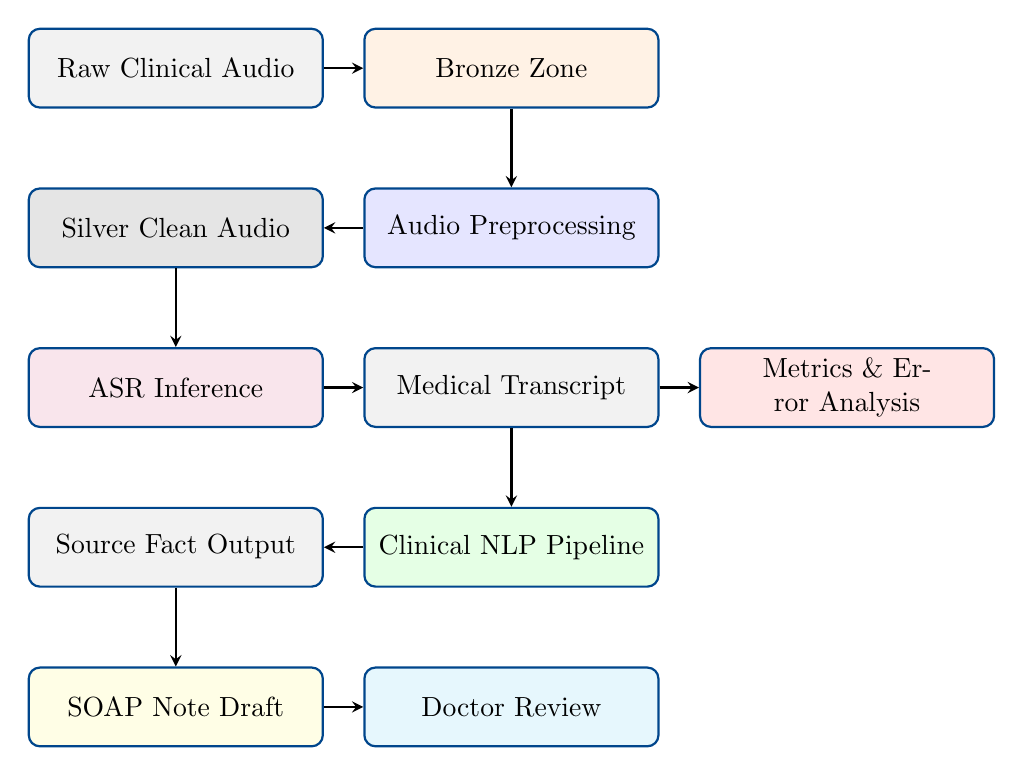
\begin{tikzpicture}[node distance=1cm and 0.5cm]
\node (A) [box, fill=gray!10] {Raw Clinical Audio};
\node (B) [box, fill=orange!10, right=of A] {Bronze Zone};
\node (C) [box, fill=blue!10, below=of B] {Audio Preprocessing};
\node (D) [box, fill=gray!20, left=of C] {Silver Clean Audio};
\node (E) [box, fill=purple!10, below=of D] {ASR Inference};
\node (F) [box, fill=gray!10, right=of E] {Medical Transcript};
\node (G) [box, fill=red!10, right=of F] {Metrics \& Error Analysis};
\node (H) [box, fill=green!10, below=of F] {Clinical NLP Pipeline};
\node (I) [box, fill=gray!10, left=of H] {Source Fact Output};
\node (J) [box, fill=yellow!10, below=of I] {SOAP Note Draft};
\node (K) [box, fill=cyan!10, right=of J] {Doctor Review};

\draw [arrow] (A) -- (B);
\draw [arrow] (B) -- (C);
\draw [arrow] (C) -- (D);
\draw [arrow] (D) -- (E);
\draw [arrow] (E) -- (F);
\draw [arrow] (F) -- (G);
\draw [arrow] (F) -- (H);
\draw [arrow] (H) -- (I);
\draw [arrow] (I) -- (J);
\draw [arrow] (J) -- (K);
\end{tikzpicture}
}
\caption{Sơ đồ tổng quan luồng xử lý Clinical Ambient Documentation Assistant}
\end{figure}

\end{document}